\NeedsTeXFormat{LaTeX2e}[2005/12/01]
%%    2011/08/29 Vorlage fuer Bachelor- und Masterarbeiten am Institut fuer Astrophysik Goettingen
%% Alle Aenderungen gegenueber der Vorlage von Thomas Pruschke (siehe unten) sind in CHANGELOG.txt im selben
%% Verzeichnis aufgelistet.
%%
%%    2009/03/12 v1.0 GAUBM Vorlage fuer Abschlussarbeiten Physik
%% Template fuer Bachelor- und Masterarbeiten
%% an der Fakultaet fuer Physik (c) Thomas Pruschke der GA Universit�t
%% Verbesserungsvorschlaege bitte an pruschke@theorie.physik.uni-goettingen.de
%%
%% Benoetigte Pakete: datenumber
%%

%%%%%%%%%%%%%%%%%%%%%%%%%%%%%%%%%%%%%%%%%%%%%%%%%%%%%%%%%%%%%%%%%%%%%%
%%%%%%%%%% Bitte vor dem Veraendern diese Datei umbenennen! %%%%%%%%%%
%%%%%%%%%%%%%%%%%%%%%%%%%%%%%%%%%%%%%%%%%%%%%%%%%%%%%%%%%%%%%%%%%%%%%%

%% scrbook - Ersatz f�r LaTeX book Klasse aus dem KOMA Script
%% Moegliche Optionen: diejenigen der Klasse scrbook ausser titlepage

%% deutsche Arbeit:
\documentclass[master,       %% Typ der Arbeit: bachelor oder master
               twoside,        %% zweiseitiges Layout
               BCOR10mm,       %% Bindekorrektur 10 mm
%               liststotoc,nomtotoc,bibtotoc, %% Aufnahme der div. Verzeichnisse
                                              %% ins Inhaltsverzeichnis
%               english,ngerman, %% Alternativspr. Englisch, Dokumentspr. Deutsch
               ngerman,english  %% Alternativspr. Deutsch, Dokumentspr. Englisch
%               final,          %% Endversion; draft fuer schnelles Kompilieren
               ]{GAUBM_astro}

\usepackage{aas_macros} %% Definiert Makros fuer Journale in Bibtex-Eintraegen von ADS

\usepackage{setspace}  %% Zur Setzung des Zeilenabstandes
\usepackage[germanb]{babel}     %% Sprachen-Unterstuetzung
\usepackage{calc}      %% ermoeglicht Rechnen mit Laengen und Zaehlern
\usepackage[T1]{fontenc}       %% Unterstutzung von Umlauten etc.
\usepackage[latin1]{inputenc}  %% 
%% in aktuellem Linux & MacOS X wird standardmaessig UTF8 kodiert!
% \usepackage[utf8]{inputenc}    %% Wenn latin1 nicht geht ...

\usepackage{amsmath,amssymb} %% zusaetzliche Mathe-Symbole

\usepackage{lmodern} %% type1-taugliche CM-Schrift als Variante zur
                     %% "normalen" EC-Schrift
%% Paket fuer bibtex-Datenbanken
\usepackage[comma,sort&compress]{natbib}
\bibliographystyle{doktor_natb_bab_amp}

\newcommand{\tabheadfont}[1]{\textbf{#1}} %% Tabellenkopf in Fett
\usepackage{booktabs}                      %% Befehle fuer besseres Tabellenlayout
\usepackage{longtable}                     %% umbrechbare Tabellen
\usepackage{array}                         %% zusaetzliche Spaltenoptionen

%% umfangreiche Pakete fuer Symbole wie \micro, \ohm, \degree, \celsius etc.
\usepackage{textcomp,gensymb}

%\usepackage{SIunits} %% Korrektes Setzen von Einheiten
\usepackage{units}   %% Variante fuer Einheiten

%% Selbst hinzugefuegte Pakete %%%%%%%%%%%%%%%%%%%%%%%%%%%%%%%%%%%%%%%%%%%%%%%%%%%%%%%%%%%%%%%%%%%%%%%%%%%%%%
\usepackage{multirow}
\usepackage{lscape}
%\usepackage{ziffer}
%\usepackage{icomma}
%\usepackage{siunitx}
\usepackage[size=normalsize]{caption}
%\usepackage[clearempty]{titlesec}

%%%%%%%%%%%%%%%%%%%%%%%%%%%%%%%%%%%%%%%%%%%%%%%%%%%%%%%%%%%%%%%%%%%%%%%%%%%%%%%%%%%%%%%%%%%%%%%%%%%%%%%%%%%%%

%% Hyperlinks im Dokument; muss als eines der letzten Pakete geladen werden
\usepackage[pdfstartview=FitH,      % Oeffnen mit fit width
            breaklinks=true,        % Umbrueche in Links, nur bei pdflatex default
            bookmarksopen=true,     % aufgeklappte Bookmarks
            bookmarksnumbered=true  % Kapitelnummerierung in bookmarks
            ]{hyperref}

%% Weiter benoetigte Pakete: datenumber
%% Falls dieses Paket nicht in der Installation vorhanden ist,
%% kann es von der Seite mit diesem Template heruntergeladen werden
%% und in einem LaTeX bekanntem Verzeichnis installiert werden (notfalls
%% dem Verzeichnis mit der Arbeit).

%% Eigene Befehle %%%%%%%%%%%%%%%%%%%%%%%%%%%%%%%%%%%%%%%%%%%%%%%%%%%%%%%%%%%%%%%%%%%%%%%%%%%%%%%%%%%%%%%%%%%
% Hier koennen nuetzliche Abkuerzungen etc. definiert werden, z.B.:
\newcommand{\ci}{\textdegree}
\newcommand{\de}{\partial}
\newcommand{\dd}{\mathrm{d}}
\newcommand{\const}{\mathrm{const.}}

%%%%%%%%%%%%%%%%%%%%%%%%%%%%%%%%%%%%%%%%%%%%%%%%%%%%%%%%%%%%%%%%%%%%%%%%%%%%%%%%%%%%%%%%%%%%%%%%%%%%%

\begin{document}
%%
%%                   Ab hier muessen die Anpassungen geschehen
%%
%% Hier den eigenen Namen einsetzen
\ThesisAuthor{Sim\'on Neftal\'i}{Torres Robledo}
%% Hier den Geburtsort einsetzen
\PlaceOfBirth{Quilitapia, Chile.}
%% Titel Arbeit. Das erste Argument ist der deutsche, das zweite der
%% englische Titel.
\ThesisTitle{Einfluss der Umgebungstemperatur auf die Wellenl\"angen stabilit\"at von $I_2$-Gaszelle}{Influence of 
Environmental Thermal Stability on the Wavelength Solution of Iodine Cells.}
%% Erst- und Zweitgutacher/in
%% Ist der/die Betreuer/in nicht identisch mit dem/r Erstgutachter/in,
%% muss diese/r als optionales Argument angegeben werden.
\FirstReferee[Prof. Dr.\ Ansgar Reiners, Dr.\ Philipp Huke]{Prof. Dr.\ Ansgar Reiners}
\Institute{Institut f\"ur Astrophysik}
\SecondReferee{Dr.\ Philipp Huke}
%% Beginn und Ende des Anfertigungszeitraumes
\ThesisBegin{1}{3}{2015}
\ThesisEnd{30}{8}{2015}
%% DO NOT TOUCH THESE LINES!!!!
\frontmatter
\maketitle
\cleardoublepage
%% Zusammenfassung. Falls nicht gewuenscht, bitte auskommentieren.

%% So laesst sich in die andere Sprache umschalten (Englisch bzw. Deutsch)
\begin{otherlanguage}{english}
\begin{abstract}
  One of the most important aspects of data analysis for astrophysics is the calibration. One technique of wavelength 
calibration for spectroscopy is using atomic standard, for instance, Molecular Iodine ($I_2$). A \emph{Gas Cell} is a 
container usually made out of glass/Pyrex in the shape of a cylinder with its interior filled with a gas. Molecular 
Iodine needs to be heated in order to be in gaseous state, from this temperature will depend the line depth (DELETE:: 
mainly and we'll see what else :: DELETE) therefore we worked on a way to have a very temperature stable Iodine$_2$ 
Cell. 
  We use a Fourier Transform Spectrograph (FTS) available at the Institute to perform 
  very high spectral resolution (R $\sim$ 600.000) measurements in order to characterize the \emph{spectral stability} in terms of line depth and wavelength
  solution. 
  \bigskip\par
  \textbf{Keywords:} Wavelength calibrators, Iodine Cells, Spectroscopy
\end{abstract}
\end{otherlanguage}

%% Ende des Vorspanns
\cleardoublepage
%% Ab hier 1 1/2 facher Zeilenabstand (durch setspace-Paket)
\onehalfspacing
%% Erzeugt Inhaltsverzeichnis
\tableofcontents

%% Hier kann man seine Bezeichnungsweisen erklaeren. Falls nicht
%% benoetigt, bis einschliesslich \end{nomenclature} auskommentieren
\begin{nomenclature}
%% Fuer die Berechnung der Spaltenbreiten muss \usepackage{calc}
%% geladen sein!
\section*{Lateinische Buchstaben}
\noindent
\begin{longtable}[l]{p{0.2\textwidth}p{0.7\textwidth-6\tabcolsep}p{0.1\textwidth}}
  \tabheadfont{Variable}&\tabheadfont{Bedeutung}&\tabheadfont{Einheit}\\\midrule\endhead
  $A$ & Querschnittsfl\"ache & $\unit{m^2}$\\
  $c$ & Geschwindigkeit & $\unitfrac{m}{s}$
\end{longtable}
\section*{Griechische Buchstaben}
\begin{longtable}[l]{p{0.2\textwidth}p{0.7\textwidth-6\tabcolsep}p{0.1\textwidth}}
  \tabheadfont{Variable}&\tabheadfont{Bedeutung}&\tabheadfont{Einheit}\\\midrule\endhead
  $\alpha$  & Winkel & $\unit{\degree}$; --\\
  $\varrho$ & Dichte & $\unitfrac{kg}{m^3}$
\end{longtable}
\section*{Indizes}
\begin{longtable}[l]{p{0.2\textwidth}p{0.8\textwidth-4\tabcolsep}}
  \tabheadfont{Index}&\tabheadfont{Bedeutung}\\\midrule\endhead
  R & Resolving Power\\
  SNR & Signal to Noise Ratio
\end{longtable}
\section*{Abk\"urzungen}
\begin{longtable}[l]{p{0.2\textwidth}p{0.8\textwidth-4\tabcolsep}}
  \tabheadfont{Abk\"urzung}&\tabheadfont{Bedeutung}\\\midrule\endhead
  FTS & Fourier Transform Spectrograph\\
  3D & dreidimensional\\
  max & maximal
\end{longtable}
\end{nomenclature}
%% \listoftables und \listoffigures sollten nur bei genuegender Anzahl Tabellen
%% verwendet werden
%\listoffigures
%\listoftables

\mainmatter   %% Anfang Hauptteil

\chapter{Introduction}
It's been a very long path since the beginning of spectroscopy, there has been 
a natural increase in the complexity of the technique.
This is only possible thanks to technological advances, in fact, science 
and technology depends on each other. Iodine cells have been in study
and use since more than a century, \cite{evans1910}. but only about two 
decades ago it has been used for \emph{precise radial velocity} measurements.

More than precise radial velocity measurements what is even more important is 
the \emph{long term stability}, specially important for the search of 
exoplanets, which at the end is precision as well but must not be confused.



\section{Motivation}
The reasons to study the influence of thermal stability on Iodine cells can be 
break down into two: First, it hasn't been done and second, the cell's 
temperature measuring methods are not very consistent therefore the gas' real 
temperature is less certain. In fact in our experiments we see that for an 
uncontrolled environment the temperature varies according to external factors 
such as: Air temperature, if the sun is hitting the window of the lab or if 
there is any source of heat in the surroundings.

From the scientific point of view the importance of this experiment is the 
benefit of knowing whether there is or not intrinsic variations in the 
wavelength solution of Iodine cells, such cells can be built with just one 
internal pressure (sealed glass tube, see Figure \ref{fig:gas-cell}) and then 
the observer controls the temperature by heating the walls of the glass and 
measuring in place. There are many drawbacks from this, for instance, the 
optical window can't be isolated therefore it is exposed to the environment. It 
will loose heat and it will always be at a lower temperature than the 
walls being heated, thus, most of the time the Iodine will condensate on the 
optical window creating black \emph{rocky} spots. This will be even more 
notorious for cells with large optical windows, say, around 5 cm or more.
%Soon after we started working it became obvious the importance of isolating 
%the experiment.

In general, besides the fact that there are many factors that will affect the 
reading, even more remarkable is the fact that the actual reading is made at 
the exterior of the cell and not inside, therefore the gas' temperature can be 
from less than one to several degrees, depending on the environment, 
cell's geometry and construction.

\section{Concepts of Spectroscopy}
Spectroscopy 
-cross section
-mean free path

\subsection{Absorption and Emission Lines}
Noch ein paar Beispiele zu Abbildungen und Tabellen:
\subsection{Line Shapes}
Atomic spectra and stability
\section{Gas Cells}
Gas Cells are glass cylinder with optical windows on its extremes. The glass 
has to be of very low thermal expansion coefficient like \emph{borosilicate} 
(Pyrex). (because is going to be glued to the optical windows therefore it would 
create mechanical tension, optical properties, reduces the risk of breaking)

\begin{figure}[h!]
 \centering
 \includegraphics[width=\columnwidth,keepaspectratio=true]{./img/gas-cell.png}
 % gas-cell.JPG: 3776x2520 pixel, 180dpi, 53.28x35.56 cm, bb=0 0 1510 1008
 \caption{The glass tube in the middle of the image is the gas cell, this one 
has angled windows in order to reduce internal reflections.}
 \label{fig:gas-cell}
\end{figure}


\subsection{Iodine}
\subsection{Other Gases}
\subsection{Cell Heating}

Heating a gas cell can be very simple as it can be challenging. It is 
easy because it is basically expose it to a controlled source of heat and it can
be challenging when we think in terms of thermal stability and in the 
potential optical effects that may occur due to thermal gradients, for instance.
In the past (citation needed) the gas cells in use are heated up until the 
line depth satisfies the observer. 
\begin{center}
 \begin{figure}[h!]
 \centering
 \includegraphics[width=\columnwidth]{./img/diag_heatloss.png}
 % diag_hardware.png: 0x0 pixel, 300dpi, 0.00x0.00 cm, bb=
 \caption{In this diagram is depicted a very rudimentary \emph{heat flow} in a simple heated gas cell system. What is clear from this is that you need
 a stable environment in order to have some stability inside the cell. Why?, because you have most of all only loss of heat.}
 \label{fig:diag_heatloss}
\end{figure}
\end{center}

It is also important that the heat distribution is homogeneous, specially at low temperatures, since iodine will crystallize in the colder parts.
the experiment of heating the cell
\begin{figure}[h!]
\centering
\includegraphics[width=\textwidth]{./img/cell_heating_idea.png}
\caption{This is the most simple method to heat up a gas cell. A wire that will heat up once an electric potential difference is placed in its extremes.}
\label{fig:cell_heating_idea}
\end{figure}
\subsubsection{A Simple Experiment}
One of the many small experiments I did while I was developing the larger one, provided me with some very clear insight on how temperature behaves in
gas cell plus heater system, and in my opinion has deep implications in the use of temperature controlled gas cells when gas temperature is critical.


\begin{figure}[h!]
 \centering
 \includegraphics[width=\textwidth]{./img/temperature_plot_2.png}
 % temperature_plot_2.png: 2400x1800 pixel, 300dpi, 20.32x15.24 cm, bb=0 0 576 432
 \caption{This experiment was made by hand, a couple of sensors placed in strategic points of an experimental cell. The dashed area corresponds to the time where power was on while
 the red vertical lines indicate the time when the outside and inside temperature reached their maximum. The dotted line is the maximum temperature inside. The dash-dotted line
 is 40 degree marker and the dashed line is the maximum obtained in the outside, which happens to be very close to the heating mechanism.}
 \label{fig:temp-plot}
\end{figure}


In the figure \ref{fig:temp-plot} you see that the interior and exterior temperatures vary in totally different ways.
Both differ in scale and timing and there is also a certain inertia, which is expected in this system. Mainly due to the insulation
that the glass provides.

In this first attempt I only wanted to see how the interior and surface temperature varied but a second extended experiment, using a very simple 
temperature control algorithm made me realize of something very important. See figure \ref{fig:simple-expe} and please take the time to identify what 
line is which. My conclusion is that this experiment, as simple as it is, demonstrates the fact that it is impossible to equalize both the exterior's and interior's
temperature if the environment is not controlled as well. This is very important because usually the cell's temperature is measured at the surface of the
cell but this value has nothing to do with the gas temperature. At this point we don't know yet how this impacts the wavelength solutions and if it does
this result is definitely very important. 
\begin{figure}[h!]
 \centering
 \includegraphics[width=\textwidth]{./img/experiment-V_012.png}
 % experiment-V_012.png: 2400x1800 pixel, 300dpi, 20.32x15.24 cm, bb=0 0 576 432
 \caption{Simple experiment demonstrate that is impossible to equalize the external cell temperature with the internal, or the gas temperature. The larger
 the difference between target and the environmental temperatures, the larger is the lag of the internal temperature compared to that of the external surface.}
 \label{fig:simple-expe}
\end{figure}

Also, this highlights the importance of TheBox experiment since we will have the air surrounding the cell, i.e. the air inside the box, the same as the 
gas' target temperature therefore we can assume that at some point the gas inside the cell will equalize to the target temperature. We could go even further
from there: We could search for empirical temperature-to-line-depth relationship and test it with measurements in uncontrolled environments.

\subsubsection{The Algorithm}
The most common controllers are the so called the PID controller: 
\chapter{Experimental Design}
Since we don't know how large is the influence of the environment in the spectral output of an Iodine Cell, the goal was to develop an stable 
environmental chamber. [[I started proposing some some crazy ideas, although I knew they were absolutely feasible, their complexity would require
much more time than what is available for a Master Thesis.]] Some of them included cell containers in which the gas cell would have been inside a 
vacuum chamber but the problem with most of them was the need of additional optical windows that would have to sustain the pressure difference
and since this have to be done by transmissive optic elements, decrease the light transmission efficiency and possibly add optic distortions by the bending due to the already mentioned difference in pressure
from the inside with the outside. The final decision was to build a box isolating the inside with foam, placing the optical elements inside and 
attempting to control the temperature. Achieving stable temperature was top priority.
\section{Hardware}
In order to achieve our goals several and diverse pieces of hardware were required, since the beginning a general idea was established but 
some of them appeared later. Figure \ref{fig:diag_hardware} shows all the hardware components and how they interact with each other,
the optical part was ignored but is well explained later. The microcomputer known as \emph{Raspberry Pi} is the core of the temperature 
control and monitoring system. The local network is also an important part because after everything was working and stable, it allowed
to monitor and control the experiment remotely.
\subsection{Optical Setup}
The idea for the optical setup was taken from an existing one used in \emph{The G\"ottingen Solar Radial Velocity Project}  by \cite{lemke2016} 
Figure \ref{fig:optical_setup} shows the general idea and the optics involved. Although the displayed setup slightly differs from the final one,
all the important optical elements are present, also the relative positions of the elements is the same.
\begin{figure}
 \centering
 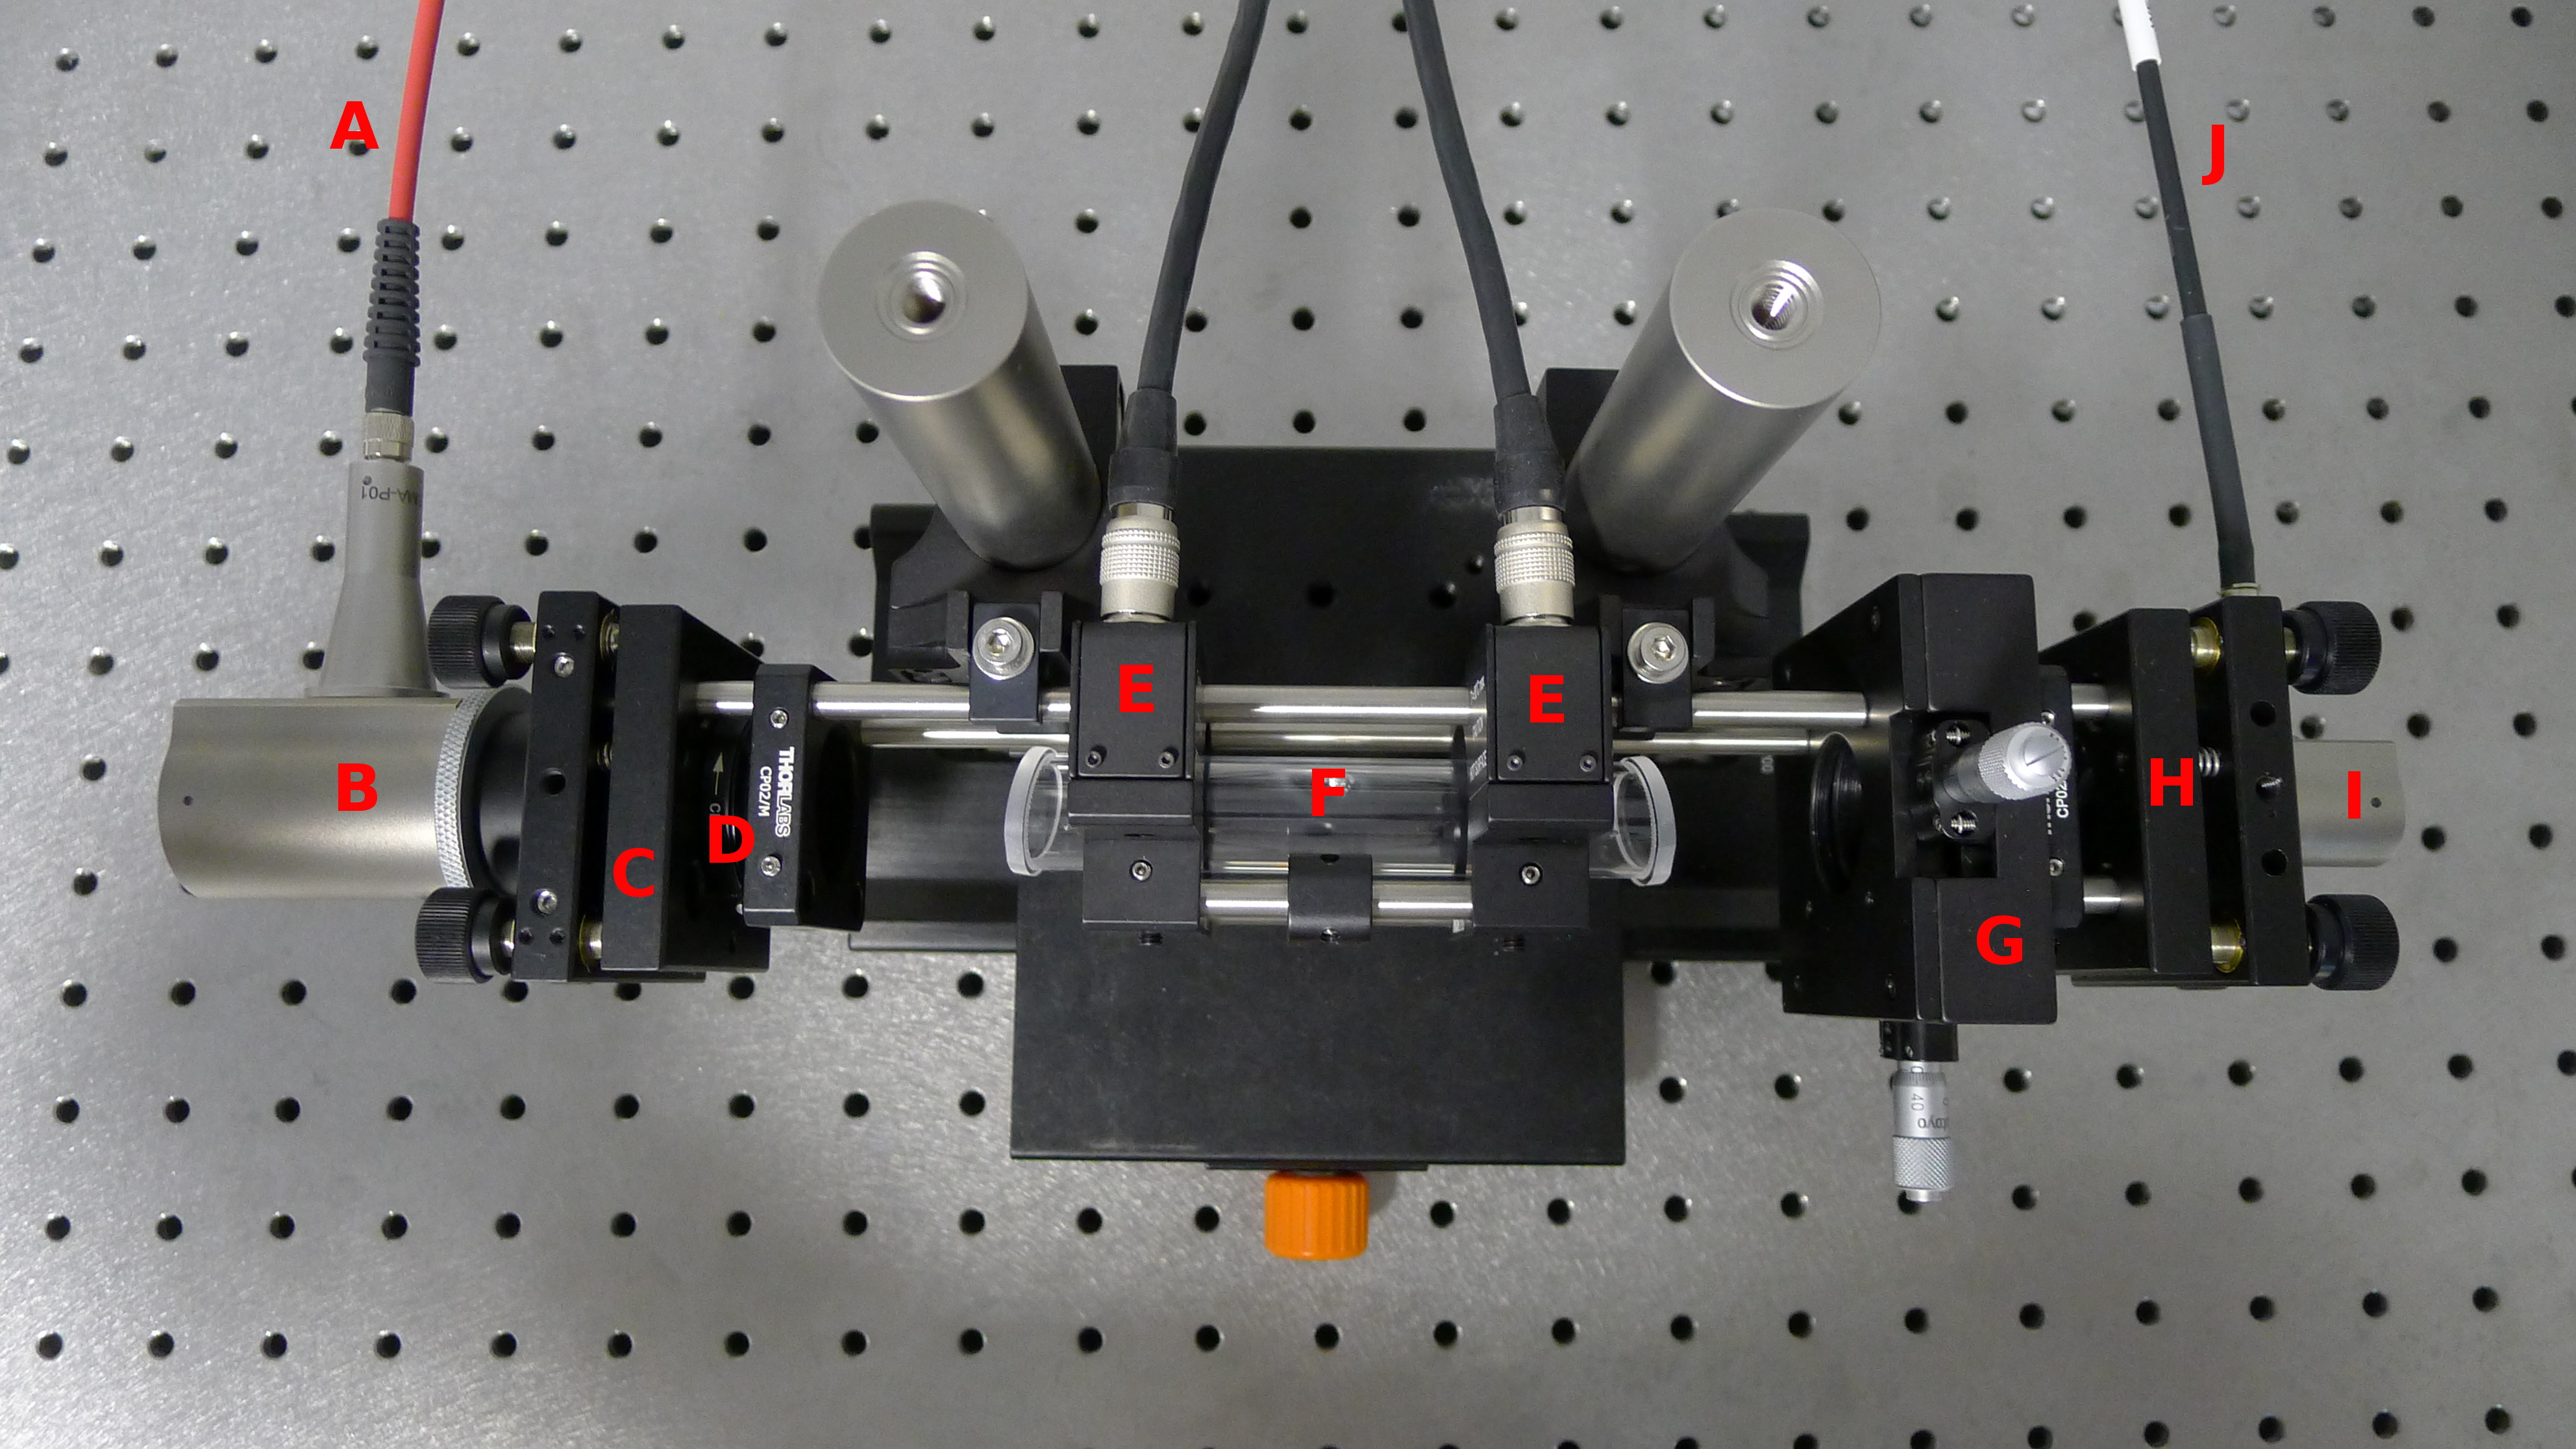
\includegraphics[width=\columnwidth,keepaspectratio=true]{./img/optical_setup_idea.jpg}
 % optical_setup_idea.jpg: 3968x2232 pixel, 180dpi, 55.99x31.50 cm, bb=0 0 1587 893
 \caption{\textbf{A:} Input optical Fiber. \textbf{B:} Reflective Collimator.  \textbf{C:} Alignment tool. \textbf{D:} Diaphragm.  \textbf{E:} Thorlabs Cell Oven. \textbf{F:} Iodine Cell.  \textbf{G:} X-Y alignment tool. \textbf{H:} Alignment tool.  \textbf{I:} Reflective Collimator. \textbf{J:} Exit Optical Fiber.}
 \label{fig:optical_setup}
\end{figure}

\subsection{TheBox}
Although the optical lab was stabilized to about 21\textdegree C, there were variations
from day to night or from sunny to cloudy days, therefore it was very necessary to make use of an extra layer of isolation, but that was not the
only motivation, we really wanted to study a very temperature-stable gas cell and have control over its temperature. Figure \ref{fig:thebox-design-appended}
shows two versions of the initial design, the base for developing the design was the needed inner volume, or in other words: the volume needed by the optical 
setup (Figure \ref{fig:optical_setup}). After, things like available materials, construction technique and costs, safety and \emph{suitability for the job} 
were considered 

\begin{figure}[h!]
\centering
\includegraphics[width=\textwidth,keepaspectratio=true]{./img/thebox_design_appended.png}
\caption{These are designs proposed to the workshop. (left) In orange you have the base and then there are screwable walls, all removable. In yellow, red, white and grey you have
the foam panels intended for thermal isolation. (right) One of the latest version of the design, but the principle is the same. At the end we allowed
the workshop decide the construction technique using this as a guide.}
\label{fig:thebox-design-appended} 
\end{figure}


\begin{figure}[h!]
\centering
\includegraphics[width=\textwidth,keepaspectratio=true]{./img/thebox.png}
\caption{The constructed box has only one opening: the top. The thicker cables pass through a specially built port. The connector with the ribbon
cable is connected to the sensors and also carries the power for the fan in the interior.}
\label{fig:thebox}
\end{figure}



\begin{figure}[h!]
\centering
\includegraphics[width=\textwidth,keepaspectratio=true,angle=90]{./img/thebox-hot-air-port.JPG}
\caption{In order to heat the air inside the box we ran a copper pipe inside, figure \ref{fig:thebox-interior}, the heat source is a 
\emph{Rework Station}, a tool used in electronics that throws  hot air through a nozzle, we let the hot air heat the pipe and the pipe heats the air inside.
We figure this is a less violent way to do it.}
\label{fig:thebox-hot-air-port}
\end{figure}


\begin{figure}[h!]
\centering
\includegraphics[width=\textwidth,keepaspectratio=true]{./img/thebox_interior.png}
\caption{This is what the interior looks like from the top. The figure \ref{fig:optical_setup} already describes the optical components. At the bottom of the image you can 
see a copper pipe, this is used as a radiator to heat up the air inside, figure \ref{fig:thebox-hot-air-port} describes how it works. At the bottom-left
there is a fan, whose function is to homogenize the temperature within the internal volume of the box. Without it there are differences of about 1
degree from side to side and up to three from top to bottom, from TheBox's perspective.}
\label{fig:thebox-interior}
\end{figure}



\subsection{Monitoring and Control}

\begin{figure}[h!]
 \centering
 \includegraphics[width=\textwidth]{./img/schema1.png}
 % schema1.png: 2838x1589 pixel, 300dpi, 24.03x13.45 cm, bb=0 0 681 381
 \caption{Schematics for Custom built Printed Circuit Board (PCB). The transistors at the bottom right were not used since they were meant for 
 serial communication between the RPI and the Arduino. Communication is done by USB. At the center you see the connector for all the temperature sensors.}
 \label{fig:schema1}
\end{figure}


\begin{figure}[h!]
 \centering
 \includegraphics[width=\textwidth]{./img/schema2.png}
 % schema1.png: 2838x1589 pixel, 300dpi, 24.03x13.45 cm, bb=0 0 681 381
 \caption{This is an independent circuit and controls the fan inside the box. It has a three-position switch. High (speed), Off and Low.
 The cables are mixed later through the only multi-pin-connector.}
 \label{fig:schema2}
\end{figure}


\begin{figure}[h!]
 \centering
 \includegraphics[width=\textwidth]{./img/board_top.png}
 % board_top.png: 1230x692 pixel, 300dpi, 10.41x5.86 cm, bb=0 0 295 166
 \caption{Top side of the printed circuit board. Not to scale.}
 \label{fig:board_top}
\end{figure}

\begin{figure}[h!]
 \centering
 \includegraphics[width=\textwidth]{./img/board_bottom.png}
 % board_top.png: 1230x692 pixel, 300dpi, 10.41x5.86 cm, bb=0 0 295 166
 \caption{Bottom side of the PCB. Not to scale.}
 \label{fig:board_bottom}
\end{figure}



\begin{figure}[h!]
 \centering
 \includegraphics[width=\textwidth]{./img/layout.png}
 % layout.png: 1230x692 pixel, 300dpi, 10.41x5.86 cm, bb=0 0 295 166
 \caption{Components placement layout.}
 \label{fig:layout}
\end{figure}


\subsubsection{Raspberry Pi}
\subsubsection{Arduino}
\subsubsection{Custom PCB}
\subsubsection{Thorlabs TC200}
\subsubsection{USB Switchbox}

\begin{center}
 \begin{figure}[h!]
 \centering
 \includegraphics[width=0.9\columnwidth]{./img/diag_hardware.png}
 % diag_hardware.png: 0x0 pixel, 300dpi, 0.00x0.00 cm, bb=
 \caption{Hardware description}
 \label{fig:diag_hardware}
\end{figure}
\end{center}



\section{Software}
\subsection{GNU/Linux}
\subsection{Python}
\subsection{Arduino}
\subsection{ZMQ}
\subsection{LAMP}
LAMP stands for: \emph{Linux, Apache, MySQL and PHP} is a widely common combinations of tools for setting up a standard 
web server
\begin{center}
 \begin{figure}[h!]
 \centering
 \includegraphics[width=0.9\columnwidth]{./img/diag_software.png}
 % diag_hardware.png: 0x0 pixel, 300dpi, 0.00x0.00 cm, bb=
 \caption{Software description}
 \label{fig:diag_software}
\end{figure}
\end{center}
\section{Instrument}
\subsection{Fourier Transform Spectrograph}
\subsection{BACHES}

\chapter{Experimental Results}




\begin{figure}[h!]
\centering
\includegraphics[width=0.5\textwidth,keepaspectratio=true]{./img/duty_cycle_example.JPG}
\caption{duty cycle example}
\label{fig:duty-cycle-example}
\end{figure}


\begin{figure}[h!]
\centering
\includegraphics[width=0.5\textwidth,keepaspectratio=true]{./img/electronics-assembled.JPG}
\caption{electronics-assembled}
\label{fig:electronics-assembled}
\end{figure}


\begin{figure}[h!]
\centering
\includegraphics[width=0.5\textwidth,keepaspectratio=true]{./img/electronics_control.png}
\caption{electronics control}
\label{fig:electronics-control}
\end{figure}


\begin{figure}[h!]
\centering
\includegraphics[width=0.5\textwidth,keepaspectratio=true]{./img/electronics-top-view.JPG}
\caption{electronics-top-view}
\label{fig:electronics-top-view}
\end{figure}


\begin{figure}[h!]
\centering
\includegraphics[width=0.5\textwidth,keepaspectratio=true]{./img/electrononics-apart.JPG}
\caption{electrononics-apart}
\label{fig:electrononics-apart}
\end{figure}



\begin{figure}[h!]
\centering
\includegraphics[width=0.5\textwidth,keepaspectratio=true]{./img/fts.JPG}
\caption{fts}
\label{fig:fts}
\end{figure}


\begin{figure}[h!]
\centering
\includegraphics[width=0.5\textwidth,keepaspectratio=true]{./img/line_detection0.png}
\caption{line detection}
\label{fig:line-detection}
\end{figure}




\begin{figure}[h!]
\centering
\includegraphics[width=0.5\textwidth,keepaspectratio=true]{./img/peltier_test.JPG}
\caption{peltier test}
\label{fig:peltier-test}
\end{figure}


\begin{figure}[h!]
\centering
\includegraphics[width=0.5\textwidth,keepaspectratio=true]{./img/thebox-casing-angle.JPG}
\caption{thebox casing angle}
\label{fig:thebox-casing-angle}
\end{figure}


\begin{figure}[h!]
\centering
\includegraphics[width=0.5\textwidth,keepaspectratio=true]{./img/thebox-casing-connections.JPG}
\caption{thebox casing connections}
\label{fig:thebox-casing-connections}
\end{figure}


\begin{figure}[h!]
\centering
\includegraphics[width=0.5\textwidth,keepaspectratio=true]{./img/thebox-casing-front.JPG}
\caption{thebox casing front}
\label{fig:thebox-casing-front}
\end{figure}






\section{Data Acquisition}
The data was obtained using the Fourier Transform Spectrograph available at the University of G\"ottingen. The following table summarizes the settings.
\subsection{Dataset}
In order to fully characterize the gas cell behavior with respect to temperature I performed the following measurements using the FTS
\begin{itemize}
 \item Stability test over 12 hours at several temperatures such as: Ambient temperature approx 22, 30, 
40, 50, 60 FTS vacuum:
 \item Heating up from ambient temperature up to 60 degree
 \item Cooling down from 60 degree to ambient temperature
 \item Long term (10 hours) measure from lab temperature up to 60 degree (too see how long does it takes to stabilize 
line depth)
\end{itemize}
\begin{center}
\begin{tabular}{|c|c|c|c|c|c|}
\hline
Temp. & Stable & Duration & FTS Vacuum & FTS Pressure (h Pa) & Date\\
\hline
30 & Yes & 5h & No & 1030.00 & 2015/08/21\\
\hline
30 & Yes & 5h & Yes & 0.262 & 2015/08/21\\
\hline
30 & Yes & 12h & Yes & 0.118 & 2015/08/22\\
\hline
40 & Yes & 12h & Yes & 0.0917 & 2015/08/24\\
\hline           
50 & Yes & 12h & Yes & 0.099 &2015/08/23 \\
\hline          
60 & Yes & 12h & Yes & 0.0917 & 2015/08/24\\
\hline
20 & No & 12h & Yes& 0.0901 &2015/08/25 \\
\hline
20-60 & Yes & 12h & Yes & 0.0779 & 2015/08/26\\
\hline              
60-20 & Yes & 12h & Yes & 0.0798 &2015/08/26 \\
\hline
%× & × & × & × & ×\\
%\hline
\end{tabular}
\end{center}


\section{Data Processing}
All the data was processed by Python scripts. It was developed in separated stages and then put together in a couple of different scripts. The next
list summarizes the key features kept in mind while developing them.
\begin{itemize}
 \item Spectral Range Cut
 \item Spline Interpolation
 \item Two Spectra Cross Correlation
 \item Line Detection
 \item Line Gaussian Fit
\end{itemize}


\textbf{Spectral Range Cut:} Selecting the spectral range is relatively easy. $wavenumber\\ cm^-1$ was the chosen unit because the data provided by
FTS data acquisition software comes natively with it. Therefore, in order to avoid error propagation from unit conversion all the process is done in wavenumber.


\textbf{Spline Interpolation} An interpolation is a mean to \emph{smooth} a data set by adding \emph{interpolated} points in between real data points.
This is helpful, for instance, in the case a signal is under sampled. Every interpolation uses a function to find the data points. 
A spline is a function (citation needed)... For this dataset a factor of twenty points was added. With the first attempt to perform a whole spectrum
spline interpolation I kept getting a MemoryError exception, because of the large amount of data being used. (add in the appendix code that worked?).

\textbf{Two Spectra Cross Correlation:} A cross correlation is used to compare two datasets in order to find similarities, in other words it could be
said that is a measure of similitude. It also possible to do self correlation in order to detect periodicity in a signal, for instance. In this case
we choose one spectrum and use it as template, usually the first of the series and then cross-correlate all the rest with respect to that one. 
There is no special reason to choose a particular one since we are interested in the relative variation and stability.

\textbf{Line Detection:} A very basic line detection algorithm is implemented, definitely improvable. The idea is to analyze very small portions of
the spectrum and measure its standard deviation. A second pass calculates the mean standard deviation of the whole spectrum and then detect 
spikes by comparing all the values to the previously calculated mean. A spike in standard deviation indicates a larger variation of the points, 
therefore the possible existence of a line. If a spike is detected a larger portion of the spectrum is covered and a minimum is obtained, 
this is used as a \emph{line candidate}. Two more conditions must be met. First is that the line candidate is at an absolute minimum and not, 
for instance, in the side of a line. An extra comparison is carried out in order to double check the previous condition. Finally, the line candidate must 
not been previously identified.

\begin{figure}
 \centering
 \includegraphics[width=\columnwidth,keepaspectratio=true]{./img/line_detection0.png}
 % line_detection0.png: 2400x1800 pixel, 300dpi, 20.32x15.24 cm, bb=0 0 576 432
 \caption{Small portion of a spectra with green vertical lines meaning successful line candidates identified. Red vertical lines are discarded line candidates. Around 23.000 line candidates are identified in the whole spectrum between 500 to 600 $nm$.}
 \label{fig:line_detection}
\end{figure}


Figure \ref{fig:line_detection} shows a very small portion of the spectrum with its lines identified. Although not all the lines 
are identified it is not a problem for us since we have thousands of lines and right now we are only interested in the most 
prominent features.

\textbf{Line Gaussian Fit:}


\section{Results}

\chapter{Future Work}

One semester is too little time to do a master thesis properly. In fact I had four month and a half of effective time to work.
The experimental setup, also named \emph{TheBox}, is ready to work stable for very long periods. The experiments performed should be repeated 
in order to 


\chapter{Discussion}


\appendix
\chapter{Appendix}
\begin{center}
 INSTRUCTIONS TO SETUP RASPBIAN FOR THE \emph{THEBOX} EXPERIMENT

\end{center}


I will assume you ''are'' using linux as a development platform, therefore I will assume
as well that you know how to open a Terminal and how to enter commands. In this document I describe roughly the steps necesary to 
get TheBox working from scratch.


 \section{Download and Install Raspbian}
    \begin{enumerate}
    \item Download the latest raspbian disk image from:
    
         \verb=     https://www.raspberrypi.org/downloads/=
    \item Identify your SD card and Install Raspbian.\\
     Before plugging the SD card in the slot type in the terminal.
     
         \verb=     > ls /dev/sd*=\\
     Observe the output, it should look something like \emph{"/dev/sda"}. Say,
     
         \verb=     /dev/sda=\\
         \verb=     /dev/sda1=\\
         \verb=     /dev/sda2=\\
         %\emph{(/dev/sdXn)}\\
     In this example, \emph{/dev/sda} is the device and \emph{/dev/sda1} and \emph{/dev/sda2} are partitions.
     Then plug the SD card and repeat the previous command, the new elements in the output
     represent your SD card. The following is an example, change accordingly.
     
         \verb=     /dev/sdb=\\
         \verb=     /dev/sdb1=\\
         \verb=     /dev/sdb2=\\
     Make sure it is unmounted by typing.
     
         \verb=     > sudo umount /dev/sdb1=\\
         \verb=     > sudo umount /dev/sdb2=\\
    \item Now you can install Raspbian. From the folder where you downloaded the raspbian image.
    
         \verb+     > sudo dd if=./raspbian-image.img of=/dev/sdb bs=4M+\\
     if you have the raspbian on a different location just give the absolute path. \verb+bs=4M+
     may sometimes not work, if that's your case try with \verb+bs=1M+
     Wait until it is finished and then remove the SD card and plug it into your Raspberry Pi.
  \end{enumerate}
  \section{Power Up and initial Setup}
  
  Power Up the Raspberry Pi by plugging a proper Power Supply Unit.
  
  \subsection{With a Screen}
%   If you are using a screen  use only this \emph{first} instruction but in the Raspberry Pi. If you are connecting from another computer 
%     you are going to discover the RPi's IP address but first you need the IP address of
%     the \emph{ETHERNET} card in the computer that you are using for development. Plug an ethernet cable between the RPi and your computer for development. 
%     Go to a terminal and type the following command.\\
    Finding your computer's IP address is very straightforward. Just open a terminal and type:\\
    \verb=     > ifconfig=\\
    The output should give you a list of the network interfaces. Look for \verb=eth0= or something like that. If you don't feel comfortably about this
    do some research with google first until you have a better idea of what you are doing. Ignore \verb=lo= and \verb=wlan0=. 
    Take pen and paper and write down this, right after \verb=inet addr:= is the IP address, please be aware that the values 
    presented here are examples only.\\
    \verb=	inet addr:192.168.0.7=\\
    You can also do this in one single command:\\
    \verb=     > ifconfig eth0 | grep 'addr:' | awk '{print $2}' \=\\
    \verb=       | sed 's/addr://g'=\\    
    If you use the previous instruction just make sure that \verb=eth0= is the actual ethernet adapter that you are using for this connection. Following 
    this example, the output should be just:\\
    \verb=	192.168.0.7=\\
  \subsection{Remotely}
  \begin{enumerate}
   
   \item If you want to work remotely, which I recommend since less resources of the Pi will be used, discovering the Raspberry Pi's IP address can be 
   a bit more dificult.
    
    Now use  \verb=nmap= in order to scan though all the possible IP addressess and discover if any is active.\\
    \verb=     > nmap -sn 192.168.0.7/24=  \\
    Unfortunately at the moment of writing this document I don't have a Raspberry Pi at hand so I just used my laptop and my current ip is 
    \textbf{ xxx.xxx.97.221}. The output will be something like this. 
    \begin{verbatim}
Starting Nmap 6.40 ( http://nmap.org ) at 2015-12-09 18:25 CLT
Nmap scan report for xxx.xxx.97.0
Host is up (0.0021s latency).
Nmap scan report for xxx.xxx.97.1
Host is up (0.0016s latency).
.
.
.
Nmap scan report for xxx.xxx.97.248
Host is up (0.0013s latency).
Nmap scan report for csp2.lco.cl (xxx.xxx.97.251)
Host is up (0.00081s latency).
Nmap done: 256 IP addresses (32 hosts up) scanned in 3.23 seconds
\end{verbatim}
    If you don't get something similar try again and if still nothing do some research on the Internet.
    Most likely you will get less entries as output. 
    
    
    When I was looking for the RPi's IP it turned out to be:\\
    \verb=     10.42.0.91=\\
    It will be easy to tell once you have the output of nmap.
    
   
    \item Next step is connect through \verb=SSH= to the RPi. The latest \emph{Raspbian} comes with SSH activated by default.\\
    \verb=     > ssh pi@10.42.0.91=\\
    The default password is \verb=raspberry=.
   \item From now on most of the commands will be on a RPi's terminal, either from a screen or from the development computer through SSH.
    If you are using a screen (and keyboard) connected to the RPi \verb=raspi-config= will pop up automatically during boot, if not type:\\
	  \verb=     > sudo raspi-config=\\

    \begin{figure}[h!]
 \centering
 \includegraphics[width=0.7\textwidth,bb=0 0 724 486]{./img/a1-raspi-config-0.png}
 % a1-raspi-config-0.png: 724x486 pixel, 72dpi, 25.54x17.15 cm, bb=0 0 724 486
 \caption{This is the first raspi-config screen, from here we will use option 1,2,5 and 9.}
 \label{fig:a1-raspi-config}
\end{figure}

%    \subsection{With a Screen}\label{sect:withscreen}
    
    \item Inital Setup with raspi-config will requiere some data which you should have at hand. Is important that you first check
    the RPi's specific documentation. Right now you will do the following steps in raspi-config
    \begin{figure}[h!]
 \centering
 \includegraphics[width=0.7\textwidth,bb=0 0 724 486]{./img/a1-raspi-config-advanced.png}
 % a1-raspi-config-advanced.png: 724x486 pixel, 72dpi, 25.54x17.15 cm, bb=0 0 724 486
 \caption{Select option 9 in the main menu to select one of the Advanced Options displayed here.}
 \label{fig:a1-raspi-config-advanced}
\end{figure}

    \begin{itemize}
     \item Expand filesystem\\ Simply hit enter in the first option and say yes to all.
     \item Set New password for user \verb=pi=\\ This is an important safety measure, option 2.
     \item Set timezone\\ Use option 5.
     \item Enable I2C\\ Use option A7, Fig. \ref{fig:a1-raspi-config-advanced}.
     
   
    \end{itemize}
    Later you will need to run raspi-config again in order to change the Hostname.
   \end{enumerate}
   
   

  \section{Advanced Setup}
  \subsection{Upgrade and Network Settings}
 \begin{enumerate}

  \item At this point we will update the repositories lists and upgrade the system to its latest stable version.\\
  \verb=     > sudo apt-get update=\\
  %\verb=     > sudo apt-get upgrade=\\
  \verb=     > sudo reboot=\\
  We do this step now because in the past this has failed so it is early enough to go back and start over, of course if it fails once I woud recommend
  not doing it next time. The current version should be already a stable one.
  \item Now the time is right to configure the network properties. I prefer to use \verb=vim= as text editor, so we will jump ahead a little bit 
  and install it. You can skip this and install or use any other text editor.\\
  \verb=     > sudo apt-get install vim=
  
  We will need to change the hostname first so we go again to \verb=raspi-config= and change the computer hostname to \verb=viscacha=.
  We don't do this the first time we run raspi-config because that causes problems when trying to login again if we haven't set the ip 
  address correctly. Remember that the information that you are about to introduce must be obtained from an authorized person of your institution.
  
  \begin{figure}[h!]
 \centering
 \includegraphics[width=0.7\textwidth,bb=0 0 724 486]{./img/a1-raspi-config-hostname.png}
 % a1-raspi-config-hostname.png: 724x486 pixel, 72dpi, 25.54x17.15 cm, bb=0 0 724 486
 \caption{hostname}
 \label{fig:a1-hostname}
\end{figure}

  
  Now edit \verb=/etc/network/interfaces=\\
  \verb=     > sudo vim /etc/network/interfaces=\\
  It should look like this:\\
  \begin{verbatim}
auto lo
iface lo inet loopback

auto eth0
allow-hotplug eth0
iface eth0 inet static

address 134.76.204.166
netmask 255.255.254.0
network 134.76.204.0
broadcast 134.76.255.255
gateway 134.76.204.254
  \end{verbatim}
  
  Beware that after this process you will not be able to access the RPi from your computer unless it is part of the internal Network of the 
  department. So is OK to leave this process to the end. Also the specific numbers might change so talk with the IT person.
  
  If you are confidant that the values are correct, reboot the pi.
\end{enumerate}

  
  \subsection{Manage Users}
  As a safety measure it is recommended to not use default values, since in that case you will be opening the gates to potential outsiders with not so good intentions.
 \begin{enumerate}
 \item Create user "thebox" \\%password 42tQb8Qa4rSHrX5
         \verb=     > sudo adduser thebox=\\
     Enter a good password when requested. Don't forget to write it somewhere.
  \item Add user to ``sudoers`` and to ``dialout'' groups.\\
         \verb=     > sudo adduser thebox sudo=\\
         \verb=     > sudo adduser thebox dialout=
  \item Allow to run \verb=sudo= commands without password (Optional). We need to edit \verb=/etc/sudoers=\\
         \verb=     > sudo visudo -f /etc/sudoers=\\
     At the end add the following line
     
         \verb+     thebox ALL=(ALL) NOPASSWD: ALL+\\
     Take advantage of the situation and delete the line corresponding to the \verb=pi= user.
     For some reason it is only possible to edit this file with the \verb=visudo= editor,
     in order to save it press \verb=Ctrl-O= and to exit \verb=Ctrl-X=. Check that the line was
     successfully added. Now you can login as \verb=thebox= and continue.
     
     \end{enumerate}
     
     \subsection{Configure SSH}
     \begin{enumerate}
   \item Create ssh public keys. You might need to do this twice, in your development computer and in your RPi.\\   
         \verb=     > ssh-keygen=\\
     My suggestion would be don't enter any passphrase because otherwise you will need to
     type in every time you want to access. Unless you need to work under the most strict security settings. No-passphrase is safe enough for now.
   See image \ref{fig:a1-ssh-keygen} for an idea of what is should look like.
     
     \begin{figure}[h!]
 \centering
 \includegraphics[width=0.7\textwidth,keepaspectratio=true]{./img/a1-ssh-keygen.png}
 % a1-ssh-keygen.png: 697x486 pixel, 72dpi, 24.59x17.15 cm, bb=0 0 697 486
 \caption{Creation of public keys.}
 \label{fig:a1-ssh-keygen}
\end{figure}

    \item Add the RPi's \verb=id_rsa.pub= to your development's \verb=authorized_keys=. and vice versa, this allows to connect without typing a password from the owner of
    \verb=id_rsa.pub= that is being pasted into \verb=authorized_keys=. Execute this command both in the Raspberry Pi and in your development computer:
    
 	\verb=     > cat ~/.ssh/id_rsa.pub | ssh user@server \=\\
 	\verb=       "cat >> ~/.ssh/authorized_keys"=\\
     where \verb=user= and \verb=server= must be changed to the proper values. I'd suggest to do it the other way around as well. From your \verb=server= or development
     computer type this:\\
     \verb=     > cat ~/.ssh/id_rsa.pub | ssh thebox@viscacha "cat \=\\
     \verb=       "cat >> ~/.ssh/authorized_keys"=\\
     Hopefully this will be the last time you type your very safe password.
     \item A very useful tool is \verb=sshfs= which allows you to mount a remote directory in your computer using \verb=ssh=. This is particularly useful when developing code.
 \end{enumerate}
 
 \section{Software Installation}
  In this section I will explain what software you need to instal and how to do it. All the programs or tools in the following list
  are required in TheBox experiment. The instalation process is tested to work in this sequence but use your criteria to tell if 
  you can alter the order. If you just updated the repositories list in the previous step is not necesary to do it again, but if many days has passed do:\\
     \verb=     > sudo apt-get update=\\
  \begin{enumerate}
   \item Install python.\\
     \verb=     > sudo apt-get install python-dev python-numpy python-scipy \=\\
     \verb=       python-matplotlib ipython=\\
  \item Install apache2 and php5  \\
     \verb=     > sudo apt-get install apache2 php5 libapache2-mod-php5=\\
  Restart apache service with:\\
     \verb=     > sudo service apache2 restart=\\
  \item Install mysql.\\
     \verb=     > sudo apt-get install mysql-server mysql-client php5-mysql \=\\
     \verb=       python-mysqldb python-mysql.connector=\\
  A password for the root user will be requested, so have it prepared or put one and write it down.
  
  If you want to edit advanced features you need to edit \verb=/etc/mysql/my.cnf=.
  
  \subsection{Configure MySQL}
  This step is very important and creates users and provide grants for them in mysql. Note that this users are not \emph{system's users} they 
  will work in MySQL's context only.
  
  \verb=     > mysql -u root -p<add password here>=\\
  Now you will get a different prompt which means that you are no longer in the operating system environment but in mysql's. So, get familiar with
  its sintaxis prior to move on.
  \begin{figure}[h!]
 \centering
 \includegraphics[width=0.7\textwidth,keepaspectratio=true]{./img/a1-mysql.png}
 % a1-mysql.png: 724x486 pixel, 72dpi, 25.54x17.15 cm, bb=0 0 724 486
 \caption{This is what you should see.}
 \label{fig:a1-mysql}
\end{figure}
\begin{enumerate}
 \item First thing to do is to create two users.
  \begin{verbatim}
CREATE USER 'thebox'@'localhost' IDENTIFIED BY '<add password here>';
CREATE USER 'vultur'@'localhost' IDENTIFIED BY '<add password here>';
\end{verbatim}
Put different passwords and take note of them.

The \emph{grant} works similar to permissions in an operating system. The user \verb=thebox= will be able to do everything on the tables but is meant to
work only from the inside of the system. On the other hand, the user \verb=vultur= will be able only to read the tables and that user can be used from
the outside, i.e. web service.
\begin{verbatim}
GRANT ALL ON *.* TO 'thebox'@'localhost';
GRANT SELECT ON *.* TO 'vultur'@'localhost';
\end{verbatim}



\item Create a database so you can place the tables.\\ \verb=CREATE DATABASE theBoxData;=\\
And then \verb=exit= MySQL.

\item If you are starting a completely new project you will not have a backup from where to restore the database, but in this case you do have one. 
Make sure to obtain the right database backup, in this case is called \verb=theboxdata.sql=.
Now import the database in the backup files to mysql.\\
\verb=     > mysql -u root -p theBoxData < theboxdata.sql=

Note that \verb=theboxdata.sql= is the name of this particular backup and it could change.


If you don't have a backup you will need to create the tables by yourself. Login as mysql root user again and type this.

\verb=USE theBoxData;=\\
This is important because it tells MySQL where to place the new table.

Make sure to type all the following text, until the semicolon.
\begin{verbatim}
 CREATE TABLE temperatureAndStatusPhaseTwo ( 
 DATE TIMESTAMP NOT NULL, 
 SENSOR_ONE DECIMAL(6,2), 
 SENSOR_TWO DECIMAL(6,2), 
 SENSOR_THREE DECIMAL(6,2), 
 SENSOR_FOUR DECIMAL(6,2), 
 SENSOR_FIVE DECIMAL(6,2), 
 SENSOR_SIX DECIMAL(6,2), 
 SENSOR_SEVEN DECIMAL(6,2), 
 TH_SET_TEMP DECIMAL(6,2), 
 TH_VAL_TEMP DECIMAL(6,2), 
 TH_HEATER_ON BOOLEAN, 
 AIR_HEATER_ON BOOLEAN
 );
\end{verbatim}


Also, when running the temperature control system, some data is stored in another table. This data is used to keep track of the current
status, should a reboot or crash happen. It will resume with the same settings afterwards.

\begin{verbatim}
CREATE TABLE thermalControl (
TSET_TIME TIMESTAMP NOT NULL, 
TSET_VALUE DECIMAL(6,2), 
LAST_HEATER_STATUS BOOLEAN
);
\end{verbatim}   
\end{enumerate}

\item Several other tools are needed:
\begin{enumerate}
 \item ZMQ is a message broadcasting system (see \verb=http://zeromq.org/=)\\
\verb=sudo apt-get install libzmq-dev python-zmq=
 \item Python Serial is needed for reading serial ports using python. Very important.\\
\verb=sudo apt-get install python-serial=
\item INO is a command line Arduino tool. Allows you to upload code into the board using command line.\\
\verb=git clone git://github.com/amperka/ino.git=\\
\verb=cd ino=\\
\verb=sudo make install=
\item The Arduino that comes in the repositories is usually an old one. Doing this is usually better. But be aware that the newest version will
be different, so I recommend you to go to \verb=www.arduino.cc= and get the correct link.\\
\verb=wget http://downloads.arduino.cc/arduino-1.6.5-linux32.tar.xz=\\
\verb=tar xf arduino-1.6.5-linux32.tar.xz=
\item Other tools needed.\\
\verb=sudo apt-get install python-rpi.gpio=\\
\verb=sudo apt-get install python-setuptools=
\end{enumerate}

\item Compile USBswitch for Raspberry Pi. The SwitchBox is an USB controled switch, you plug it to a wall power outlet and then conect to it a
device that you want to control. In order to control you need to send a signal through an USB port, since the protocol for sending such instructions are
too complicated to developt one's own code it is easier to use their example but it comes pre-compiled for \verb=i386= architecture, therefore is necessary
to compile it for the \verb=ARM= arquitecture.\\
First install the necessary libraries:\\
\verb=     > sudo apt-get install libusb-dev=\\
\verb=     > sudo apt-get install libstdc++6=\\
\verb=     > sudo apt-get install libc6=\\
\verb=     > sudo apt-get install libgcc1=\\
Go to SwitchBox manufacturer's webpage  \\
\verb=http://www.antrax.de=\\
Search for the product's page of the SwitchBox device and click the \emph{Downloads} tab and then click on \emph{linux}.
Save the file and unpack it with:\\
\verb=     > mkdir antrax=\\
\verb=     > cd antrax=\\
\verb=     > unzip ../switchboxusb-linux.zip=\\
\verb=     > unzip AntraxAccess.zip=\\
\verb=     > unzip AntraxLinux.zip=\\

You will find a \emph{pdf} document with instructions in German: \verb=Switchbox-USB-Linux.pdf=\\
%This comes precompiled for \verb=i386=. We need to compile it for \verb=ARM=.\\
In order to proceed to the compilation, do the following:\\
\verb=     > cd USBaccess=\\
\verb=     > vim USBaccessBasic.c=\\
Change the line \verb=14= from \verb=#include <linux/usb.h>= to \verb=#include <usb.h>=\\
\verb=     > cc -c -lusb -o USBaccessBasic.o USBaccessBasic.c=\\
\verb=     > rm USBaccess.o=\\
\verb=     > make=\\
\verb=     > cp USBaccess.a USBaccess.h USBaccess.o ../Example/=\\
\verb=     > cd ../Example=\\
\verb=     > rm USBswitch USBswitch.o=\\
\verb=     > make=\\
At this point the command-line tool is ready to work but some work is still needed.\\
\verb=     > ls /dev/usb/=\\
The output should show something like this:\\
\verb=       hiddev0 hiddev1=\\
If nothing comes out is likely that \verb=udevd= is not working. It's possible to find out by typing:\\
\verb=     > pidof udevd=\\
Create a new rule. I think the best way proceed is as follows:\\
\verb#     > sudo echo 'BUS=="usb", KERNEL=="hiddev[0-9]", NAME="usb/hiddev%n",\#\\ 
\verb# MODE="0666"' >> /etc/udev/rules.d/10-local.rules#\\
If it doesn't work type \verb=sudo su= and you will be root. Now you can run the previous command.
Restart the service:\\
\verb=     > sudo /etc/init.d/udev restart=\\
\verb=     > cd USBaccess=\\
\verb=     > source make_hid=\\
By default we need to run \verb=USBswitch= as \verb=root= or with \verb=sudo=, this is just a matter of permissions but is not a good
idea just to change the permissions of the device. Do the following:\\
\verb=     > sudo chmod g+rw /dev/usb/hiddev0=\\
\verb=     > sudo  chgrp dialout /dev/usb/hiddev0=\\
Now you can turn on or off the SwitchBox.\\
\verb=     > USBswitch 1= (on)\\
\verb=     > USBswitch 0= (off)\\
After a reboot the permissions of the file \verb=/dev/usb/hiddev0= will return to normal so you might need to do this everytime. A script exists in the
latest system called \verb=setUSBswitch=.

\section{Adding a Real Time Clock (RTC)}
Since the Raspberry Pi is meant to be a cheap computer it doesn't come with an internal clock, so its recomended to use an RTC.
There is one implemented that uses the I2C protocol. \\
\verb=sudo apt-get install python-smbus=\\
\verb=sudo apt-get install i2c-tools=

We will need adafruit's instructions to setup correctly the RTC.\\
\verb=https://learn.adafruit.com/adding-a-real-time\=\\
\verb=-clock-to-raspberry-pi/overview=\\
The following instructions are reproduced from there, I will asume you have a revision 2 Raspberry Pi. At this point the RTC should be already pluged correctly.
In order to verify that, type:

\verb=     > sudo i2cdetect -y 1=

\begin{figure}
 \centering
 \includegraphics[width=0.7\textwidth]{./img/a1-i2cdetect.png}
 % i2cdetect.png: 472x252 pixel, 72dpi, 16.65x8.89 cm, bb=0 0 472 252
 \caption{This is what you should see. If instead of 68 you get UU, it means that the RTC has already been setup.}
 \label{fig:i2cdetect}
\end{figure}

If everything is working fine, move to the next level. First load the RTC kernel module:\\
\verb=     > sudo  modprobe rtc-ds1307=\\
Then you will need to be root, in raspbian (or any debian distro) the following instruction makes you root.\\
\verb=     > sudo su=\\
\verb=     > echo ds1307 0x68 > /sys/class/i2c-adapter/i2c-1/new_device=\\
Type \verb=exit= to go back to your normal user.

Check the time of the RTC with \verb=sudo hwclock -r= and if it is the first time this has been done you should get the 1st of January of 2000.

Check the time of your Raspberry Pi with \verb=date= If it is not correct run \verb=sudo raspi-config= and set the right timezone, if you are conected
to the internet that should fix the time properly. Now check the time again with \verb=date= and then write it to the RTC.

\verb=     > sudo hwclock -w= 

Again, you can check it with:

\verb=     > sudo hwclock -r=

If everything is correct at this point it means you have a running RTC, but at the next reboot it will not be working so we need to make the RTC kernel
module to load at boot time.

\verb=     > sudo vim /etc/modules=\\
At the end of the file add \verb=rtc-ds1307=

Now for the creation of the RTC device at boot time edit \verb=/etc/rc.local=\\

\verb=     > sudo vim /etc/rc.local=

Add, \emph{BEFORE} \verb=exit 0=.\\
\verb=echo ds1307 0x68 > /sys/class/i2c-adapter/i2c-1/new_device=\\
\verb=sudo hwclock -s=

\begin{figure}[h!]
 \centering
 \includegraphics[width=0.7\textwidth,keepaspectratio=true]{./img/a1-rc-local.png}
 % rc-local.png: 634x486 pixel, 72dpi, 22.37x17.15 cm, bb=0 0 634 486
 \caption{This is what the file \emph{/etc/rc.local} should look like.}
 \label{fig:rc-local}
\end{figure}

\end{enumerate}

\section{Webpage} [this part on neeeds some work]
Place the webfiles in \verb=/var/www/http/=
\section{TheBox Control Software}
\verb=     > mkdir ~/.bin=\\
Move the files there\\
edit \verb=.bashrc=\\
\verb=     > vim .bashrc=\\
add the line\\
\verb+export PATH=$PATH:/home/thebox/.bin+
\section{Clean Up}
bllbala

\chapter{zweiter Anhang}
Text\dots

\cleardoublepage
%% Bibliographie. Das Argument muss der Name der BIBTeX-Datenbank stehen.
%% Ein Beispiel fuer eine solche Datenbank finden Sie in bthesis_datenbank.bib
\bibliography{iodine} 

\chapter*{Danksagung}
Thanks
%% Dieser Befehl MUSS am Ende stehen und erzeugt die Erklaerung ueber die
%% benutzten Mittel
\Declaration
\end{document}
